\section{Is quantum computing a treat to blockchains' security?}

Now that we have a better idea of how a quantum computer works, let's try to figure out how to hack mining process with a quantum computer (see \cite{quantum_computer}). \newline

For recall, the goal of mining is to find a nonce so the hash is lower than a specific target. The nonce is a 4-bytes value, so to use quantum computers to solve this problem, we'll need 4 qubytes or 32 qubits. A block header is 80 bytes so we'll append the 4 qubytes to 76 regular bytes and we'll get a 256 bits result.\newline

Nowadays, quantum computers are not as easy to program as classic computers because quantum computers don't use the same logic gates so we'll need to build the circuit corresponding to our algorithm.

\clearpage

\begin{figure}[ht]
\centering
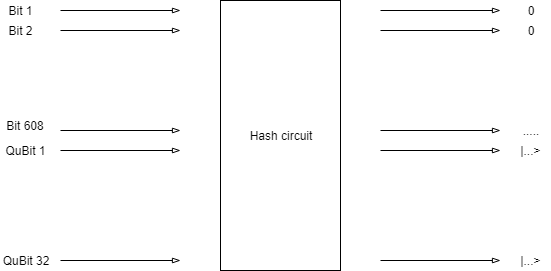
\includegraphics[width=12cm]{Figures/hashCircuit}
\caption{Circuit to build to hack mining}
\end{figure}
\medskip

But here we have a problem, with a quantum computer, it's quite easy to find the final hash lower than the target but, due to the wave function collapse, we can't find which value of the nonce gave this output but it's exactly what we're looking for. \newline

With the qubits, we can simultaneously have all the hashes with all the possible values of the nonce. To find the right ones, we could loop through all the solutions but it won't be faster than traditional mining so it's back to square one.

\subsection{Grover algorithm}

A solution to this problem is Grover algorithm (see \cite{groverWiki}) which reduces the complexity to search in N values from $\mathcal{O}(N)$ to $\mathcal{O}(\sqrt{N})$. \newline

The goal is to find a solution in a list of N values, the solution is defined by a function f where:

\[
  f(x) =
  \begin{cases}
    1, & \text{if it's the solution}  \\
    0, & \text{otherwise} \\
  \end{cases}
\]
\medskip

We have a list of N values so the numbers can be described this way:

\begin{equation}
  \begin{aligned}
    \bra{\Psi} &= c_0 . \bra{00...0} + c_1 . \bra{00...1} + ... + c_{N-1} . \bra{11...1}
    &= \sum_{i=0}^{N-1} c_i . \bra{i}
  \end{aligned}
\end{equation}

where $\sum_{i=0}^{N-1} | c_i |^2 = 1$. \newline

Grover algorithm follows these steps: \newline

\begin{enumerate}
  \item It creates a uniform superposition over all states: \newline

  $\bra{\Psi}_{initial} = \frac{1}{\sqrt{N}} \sum_{i=0}^{N-1} \bra{i}$ \newline

  (We would like $\bra{\Psi}_{final} = \epsilon . \bra{00...0} + ... + (1 - \epsilon) . \bra{solution} + ... + \epsilon . \bra{11...1}$)

  \item It applies an operator to inverse the phase of the solutions.
  \item It applies an operator to increase and decrease magnitudes, it corresponds to a mirror of magnitudes around their mean.
  \item It repeats the two last steps $\approx \frac{\pi}{4} \sqrt(N)$

\end{enumerate}
\medskip

Next some schemes to illustrate the steps:

\clearpage

\begin{figure}[ht]
\centering

\subfloat[Step 1]{
  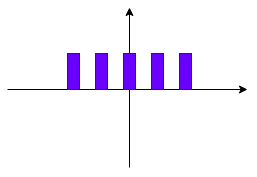
\includegraphics[width=6cm]{Figures/step1}
}
\hspace{1cm}
\subfloat[Step 2]{
  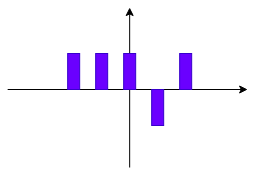
\includegraphics[width=6cm]{Figures/step2}
}
\end{figure}
\medskip

\begin{figure}[ht]
\centering

\subfloat[Step 3]{
  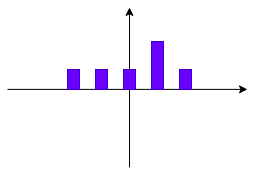
\includegraphics[width=6cm]{Figures/step3}
}
\hspace{1cm}
\subfloat[Step 4 (after all iterations)]{
  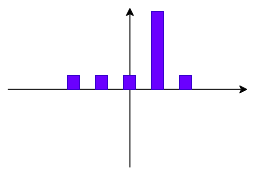
\includegraphics[width=6cm]{Figures/step4}
}
\end{figure}
\medskip

Now, with this algorithm, we can reduce the complexity to $\mathcal{O}(\sqrt{N})$. In our case, we have 32 qubits so there are $N = 2^{32}$ possible values then we have to search in $\sqrt(N) = \sqrt{2^{32}} = 2^{16} = 65,536$. \newline

With this method, we have a theoretical solution to hack mining with a quantum computer, so it proves that quantum computing could be a real treat to blockchains security. It will depend on the evolution in the quantum field and the researches to improve the performances and stability of quantum computers.
